
\begin{figure}
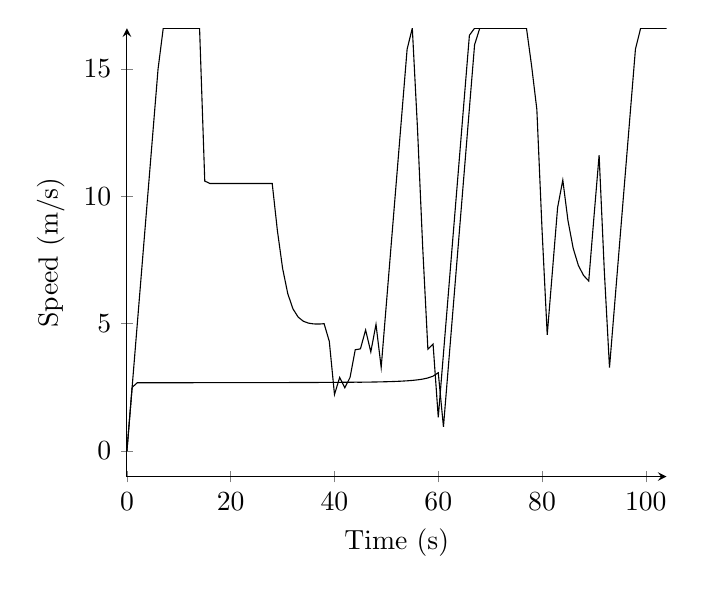
\begin{tikzpicture}
\begin{axis}[
legend style={anchor=west},
axis x line=bottom,
axis y line=left,
ymin=-1,
xlabel=Time (s),
ylabel=Speed (m/s),
]
\addplot[] coordinates {
(0, 0.0)
(1, 2.5)
(2, 2.68300447108)
(3, 2.68309840976)
(4, 2.68319688255)
(5, 2.68330018636)
(6, 2.68340864281)
(7, 2.68352260077)
(8, 2.6836424392)
(9, 2.68376857028)
(10, 2.68390144301)
(11, 2.68404154723)
(12, 2.68418941815)
(13, 2.6843456415)
(14, 2.68451085938)
(15, 2.68468577691)
(16, 2.68487116978)
(17, 2.68506789299)
(18, 2.68527689073)
(19, 2.68549920783)
(20, 2.68573600294)
(21, 2.6859885638)
(22, 2.68625832487)
(23, 2.68654688798)
(24, 2.68685604634)
(25, 2.68718781274)
(26, 2.68754445271)
(27, 2.68792852373)
(28, 2.68834292168)
(29, 2.68879093621)
(30, 2.68927631712)
(31, 2.68980335398)
(32, 2.69037697263)
(33, 2.69100285237)
(34, 2.69168756925)
(35, 2.69243877244)
(36, 2.69326540261)
(37, 2.69417796425)
(38, 2.69518886799)
(39, 2.69631286409)
(40, 2.69756759653)
(41, 2.69897431763)
(42, 2.70055881937)
(43, 2.70235266045)
(44, 2.70439480294)
(45, 2.70326388413)
(46, 2.70589594061)
(47, 2.70903544021)
(48, 2.71271306005)
(49, 2.71706157312)
(50, 2.72225830602)
(51, 2.72854483077)
(52, 2.73625791401)
(53, 2.74587997166)
(54, 2.75812500553)
(55, 2.77409302159)
(56, 2.79556675528)
(57, 2.82563361416)
(58, 2.87015208609)
(59, 2.94184965083)
(60, 3.07535912664)
(61, 0.951044378225)
(62, 3.45104437822)
(63, 5.95104437822)
(64, 8.45104437822)
(65, 10.9510443782)
(66, 13.4510443782)
(67, 15.9510443782)
(68, 16.6)
(69, 16.6)
(70, 16.6)
(71, 16.6)
(72, 16.6)
(73, 16.6)
(74, 16.6)
(75, 16.6)
(76, 16.6)
(77, 16.6)
(78, 15.1057186669)
(79, 13.409293294)
(80, 8.69044405884)
(81, 4.56048379288)
(82, 7.06048379288)
(83, 9.56048379288)
(84, 10.6384312281)
(85, 9.04461055735)
(86, 7.96313700813)
(87, 7.28818661487)
(88, 6.89504423037)
(89, 6.67699879493)
(90, 9.17699879493)
(91, 11.618896522)
(92, 7.07664927985)
(93, 3.27787502772)
(94, 5.77787502772)
(95, 8.27787502772)
(96, 10.7778750277)
(97, 13.2778750277)
(98, 15.7778750277)
(99, 16.6)
(100, 16.6)
(101, 16.6)
(102, 16.6)
(103, 16.6)
(104, 16.6)
};
\addplot[] coordinates {
(0, 0.0)
(1, 2.5)
(2, 5.0)
(3, 7.5)
(4, 10.0)
(5, 12.5)
(6, 15.0)
(7, 16.6)
(8, 16.6)
(9, 16.6)
(10, 16.6)
(11, 16.6)
(12, 16.6)
(13, 16.6)
(14, 16.6)
(15, 10.6)
(16, 10.5046972585)
(17, 10.5047257482)
(18, 10.5047584871)
(19, 10.5047963643)
(20, 10.5048405148)
(21, 10.504892405)
(22, 10.5049539562)
(23, 10.5050277261)
(24, 10.5051171783)
(25, 10.5052270978)
(26, 10.505364246)
(27, 10.505538428)
(28, 10.5057643014)
(29, 8.6497712866)
(30, 7.17240237095)
(31, 6.1769229136)
(32, 5.58152935882)
(33, 5.25900876564)
(34, 5.09709939141)
(35, 5.02163613053)
(36, 4.99144904783)
(37, 4.9863267896)
(38, 4.99999089821)
(39, 4.3074265869)
(40, 2.22124471293)
(41, 2.88978317051)
(42, 2.48586988488)
(43, 2.89245303915)
(44, 3.97661314563)
(45, 4.01318107553)
(46, 4.7528745596)
(47, 3.8929184844)
(48, 4.97428056348)
(49, 3.28321977261)
(50, 5.78321977261)
(51, 8.28321977261)
(52, 10.7832197726)
(53, 13.2832197726)
(54, 15.7832197726)
(55, 16.6)
(56, 12.652247739)
(57, 8.00283445772)
(58, 4.00226771076)
(59, 4.19696753101)
(60, 1.32219478411)
(61, 3.82219478411)
(62, 6.32219478411)
(63, 8.82219478411)
(64, 11.3221947841)
(65, 13.8221947841)
(66, 16.3221947841)
(67, 16.6)
(68, 16.6)
(69, 16.6)
(70, 16.6)
(71, 16.6)
};

\end{axis}
\end{tikzpicture}
\label{tik:100:2_O, 2_O.-60, 4_S, 5_S, 5_S.-30, 7_S, 7_S.-25, 10_O}
\caption{100 percent diving with GSC on route $2_O, 2_O.-60, 4_S, 5_S, 5_S.-30, 7_S, 7_S.-25, 10_O$}
\end{figure}
